% $Header: /Users/joseph/Documents/LaTeX/beamer/solutions/conference-talks/conference-ornate-20min.en.tex,v 90e850259b8b 2007/01/28 20:48:30 tantau $

\documentclass{beamer}

% This file is a solution template for:

% - Talk at a conference/colloquium.
% - Talk length is about 20min.
% - Style is ornate.



% Copyright 2004 by Till Tantau <tantau@users.sourceforge.net>.
%
% In principle, this file can be redistributed and/or modified under
% the terms of the GNU Public License, version 2.
%
% However, this file is supposed to be a template to be modified
% for your own needs. For this reason, if you use this file as a
% template and not specifically distribute it as part of a another
% package/program, I grant the extra permission to freely copy and
% modify this file as you see fit and even to delete this copyright
% notice. 


\mode<presentation>
{
  \usetheme{CambridgeUS}
  % or ...

  \setbeamercovered{transparent}
  % or whatever (possibly just delete it)
  
\makeatletter
\setbeamertemplate{footline}
{
  \leavevmode%
  \hbox{%
  \begin{beamercolorbox}[wd=.333333\paperwidth,ht=2.25ex,dp=1ex,center]{author in head/foot}%
    \usebeamerfont{author in head/foot}Salvatore Aiola
   \end{beamercolorbox}%
  \begin{beamercolorbox}[wd=.333333\paperwidth,ht=2.25ex,dp=1ex,center]{title in head/foot}%
    \usebeamerfont{title in head/foot}\insertshorttitle
  \end{beamercolorbox}%
  \begin{beamercolorbox}[wd=.333333\paperwidth,ht=2.25ex,dp=1ex,right]{date in head/foot}%
    \usebeamerfont{date in head/foot}\insertshortdate{}\hspace*{2em}
    \insertframenumber{} / \inserttotalframenumber\hspace*{2ex} 
  \end{beamercolorbox}}%
  \vskip0pt%
}
\setbeamertemplate{headline}{%
\leavevmode%
  \hbox{%
    \begin{beamercolorbox}[wd=.5\paperwidth,ht=2.25ex,dp=1ex]{section in head/foot}%
    \usebeamerfont{section in head/foot}\,\insertsection
    \end{beamercolorbox}%
    \begin{beamercolorbox}[wd=.5\paperwidth,ht=2.25ex,dp=1ex,right]{subsection in head/foot}%
    \usebeamerfont{section in head/foot}The ALICE Collaboration\,
    \end{beamercolorbox}%
  }
}
\makeatother
}


\usepackage[english]{babel}
% or whatever

\usepackage[latin1]{inputenc}
% or whatever

\usepackage{times}
\usepackage[T1]{fontenc}
% Or whatever. Note that the encoding and the font should match. If T1
% does not look nice, try deleting the line with the fontenc.
%particles
\newcommand{\jpsi}{\rm J/$\psi$}
\newcommand{\psip}{$\psi^\prime$}
\newcommand{\jpsiDY}{\rm J/$\psi$\,/\,DY}
\newcommand{\chic}{$\chi_{\rm c}$}
\newcommand{\pip}{$\pi^{+}$}
\newcommand{\pim}{$\pi^{-}$}
\newcommand{\pizero}{$\pi^{0}$}
\newcommand{\kap}{K$^{+}$}
\newcommand{\kam}{K$^{-}$}
\newcommand{\pbar}{$\rm\overline{p}$}
\newcommand{\ccbar}{\ensuremath{\mathrm{c\overline{c}}}}
\newcommand{\bbbar}{\ensuremath{\mathrm{b\overline{b}}}}
\newcommand{\Dzero}{\ensuremath{\mathrm{D^{0}}}}
\newcommand{\Dzerobar}{\ensuremath{\mathrm{\overline{D}^{0}}}}
\newcommand{\Dpm}{\ensuremath{\mathrm{D^{\pm}}}}
\newcommand{\Ds}{\ensuremath{\mathrm{D_{s}^{\pm}}}}
\newcommand{\Dstar}{\ensuremath{\mathrm{D^{*\pm}}}}

%collision systems
\newcommand{\pp}{pp}
\newcommand{\pPb}{p--Pb}
\newcommand{\PbPb}{Pb--Pb}

%detectors
\newcommand{\ezdc}{$E_{\rm ZDC}$}

%units
\newcommand{\GeVc}{GeV/$c$}
\newcommand{\GeVcsq}{GeV/$c^2$}

%others
\newcommand{\degree}{$^{\rm o}$}
\newcommand{\s}{\ensuremath{\sqrt{s}}}
\newcommand{\snn}{\ensuremath{\sqrt{s_{\rm NN}}}}
\newcommand{\y}{\ensuremath{y}}
\newcommand{\pt}{\ensuremath{p_{\rm T}}}
\newcommand{\dedx}{d$E$/d$x$}
\newcommand{\dndy}{d$N$/d$y$}
\newcommand{\dndydpt}{${\rm d}^2N/({\rm d}y {\rm d}p_{\rm t})$}
\newcommand{\zpar}{\ensuremath{z_{||}}}
\newcommand{\zpargen}{\ensuremath{z_{||}^{\mathrm{part}}}}
\newcommand{\zpardet}{\ensuremath{z_{||}^{\mathrm{det}}}}
\newcommand{\ptchjet}{\ensuremath{p_{\mathrm{T,ch\, jet}}}}
\newcommand{\ptjet}{\ensuremath{p_{\mathrm{T,jet}}}}
\newcommand{\ptchjetgen}{\ensuremath{p_{\mathrm{T,ch\,jet}}^{\mathrm{truth}}}}
\newcommand{\ptchjetdet}{\ensuremath{p_{\mathrm{T,ch\,jet}}^{\mathrm{reco}}}}
\newcommand{\ptd}{\ensuremath{p_{\mathrm{T,D}}}}
\newcommand{\ptdgen}{\ensuremath{p_{\mathrm{T,D}}^{\mathrm{truth}}}}
\newcommand{\ptddet}{\ensuremath{p_{\mathrm{T,D}}^{\mathrm{reco}}}}
\newcommand{\antikt}{anti-\ensuremath{k_{\mathrm{T}}}}
\newcommand{\kt}{\ensuremath{k_{\mathrm{T}}}}
\newcommand{\pthard}{\ensuremath{p_{\mathrm{T,hard}}}}

\title[D-tagged jets in pp collisions at 7 TeV] % (optional, use only with long paper titles)
{D-meson tagged jets in pp collisions at 7 TeV}

\author% (optional, use only with lots of authors)
{Salvatore Aiola (Yale University),\\
on behalf of the ALICE Collaboration\\
\bigskip

\includegraphics[height=2cm]{img/yale}\quad
\includegraphics[height=2cm]{img/alice}}
% - Give the names in the same order as the appear in the paper.
% - Use the \inst{?} command only if the authors have different
%   affiliation.

\institute[Yale University] % (optional, but mostly needed)


\date[Hot Quarks 2016] % (optional, should be abbreviation of conference name)
{Hot Quarks 2016, September 12-17, South Padre Island, TX}
% - Either use conference name or its abbreviation.
% - Not really informative to the audience, more for people (including
%   yourself) who are reading the slides online

\subject{High-Energy Physics}
% This is only inserted into the PDF information catalog. Can be left
% out. 



% If you have a file called "university-logo-filename.xxx", where xxx
% is a graphic format that can be processed by latex or pdflatex,
% resp., then you can add a logo as follows:

% \pgfdeclareimage[height=0.5cm]{university-logo}{university-logo-filename}
% \logo{\pgfuseimage{university-logo}}


% If you wish to uncover everything in a step-wise fashion, uncomment
% the following command: 

%\beamerdefaultoverlayspecification{<+->}


\begin{document}

\begin{frame}
  \titlepage
\end{frame}

\begin{frame}{Outline}
  \tableofcontents
  % You might wish to add the option [pausesections]
\end{frame}


% Structuring a talk is a difficult task and the following structure
% may not be suitable. Here are some rules that apply for this
% solution: 

% - Exactly two or three sections (other than the summary).
% - At *most* three subsections per section.
% - Talk about 30s to 2min per frame. So there should be between about
%   15 and 30 frames, all told.

% - A conference audience is likely to know very little of what you
%   are going to talk about. So *simplify*!
% - In a 20min talk, getting the main ideas across is hard
%   enough. Leave out details, even if it means being less precise than
%   you think necessary.
% - If you omit details that are vital to the proof/implementation,
%   just say so once. Everybody will be happy with that.

\section{Physics Motivations}

\subsection{Heavy-Flavor and pQCD}
\begin{frame}{Heavy-Flavor and pQCD}
\centering
\includegraphics[width=.4\paperwidth]{img/ALICE_D0Meson}
\quad
\includegraphics[width=.42\paperwidth]{img/ATLAS_DStarJets}
\end{frame}

\subsection{Heavy-Flavor and the QGP}
\begin{frame}{Heavy-Flavor and the QGP}
\centering
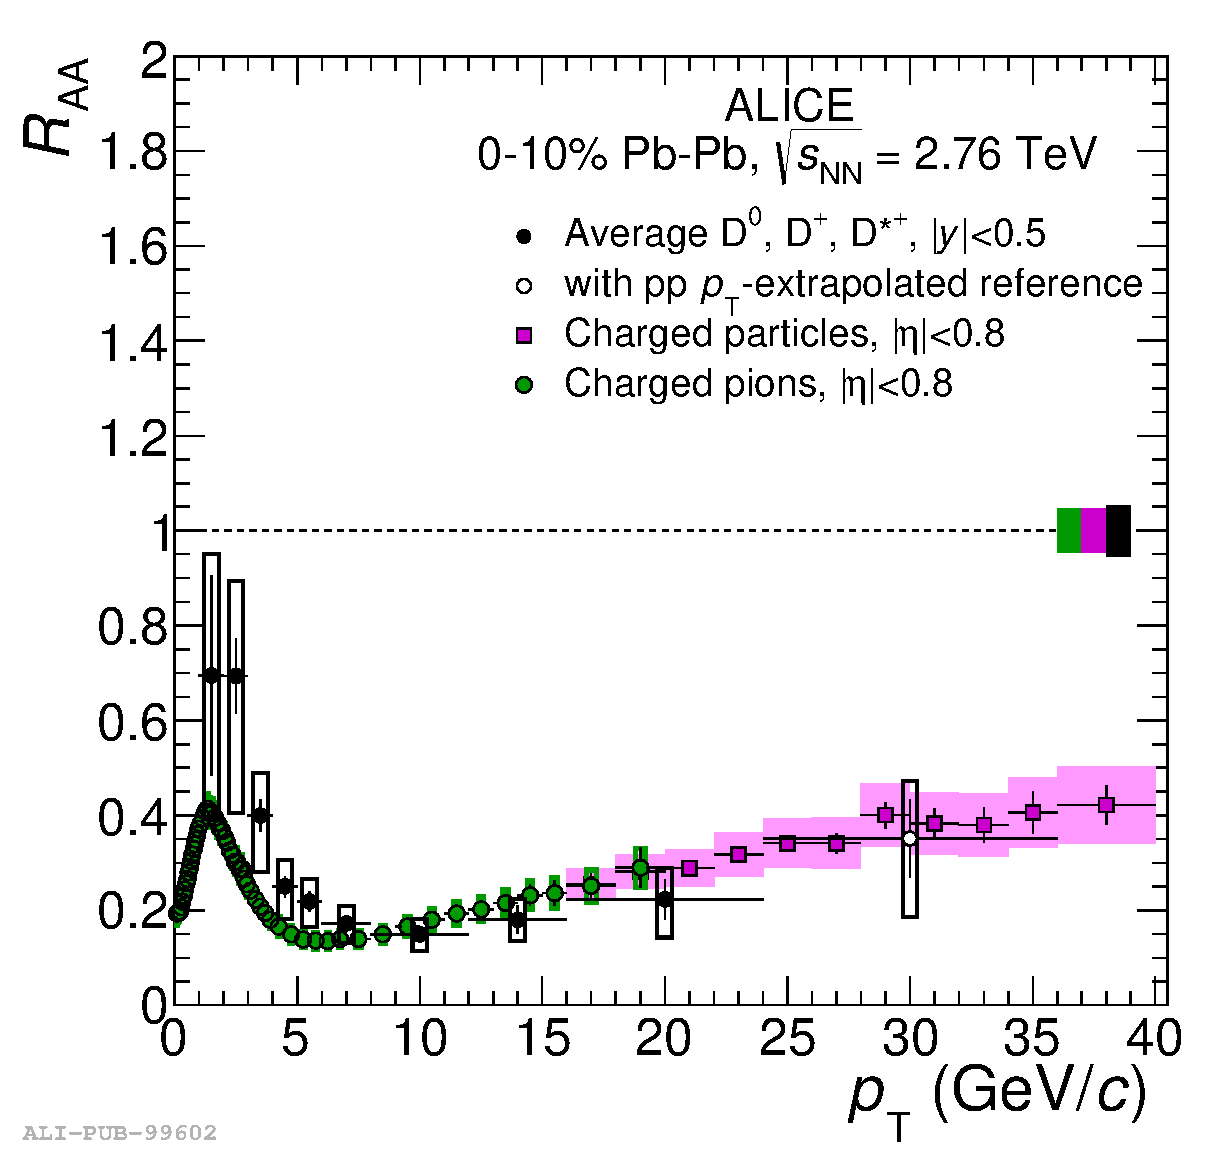
\includegraphics[width=.4\paperwidth]{img/ALICE_DMesonRAA}
\end{frame}

\section{Analysis Overview}

\subsection{ALICE at the LHC}
\begin{frame}{ALICE at the LHC}
\centering
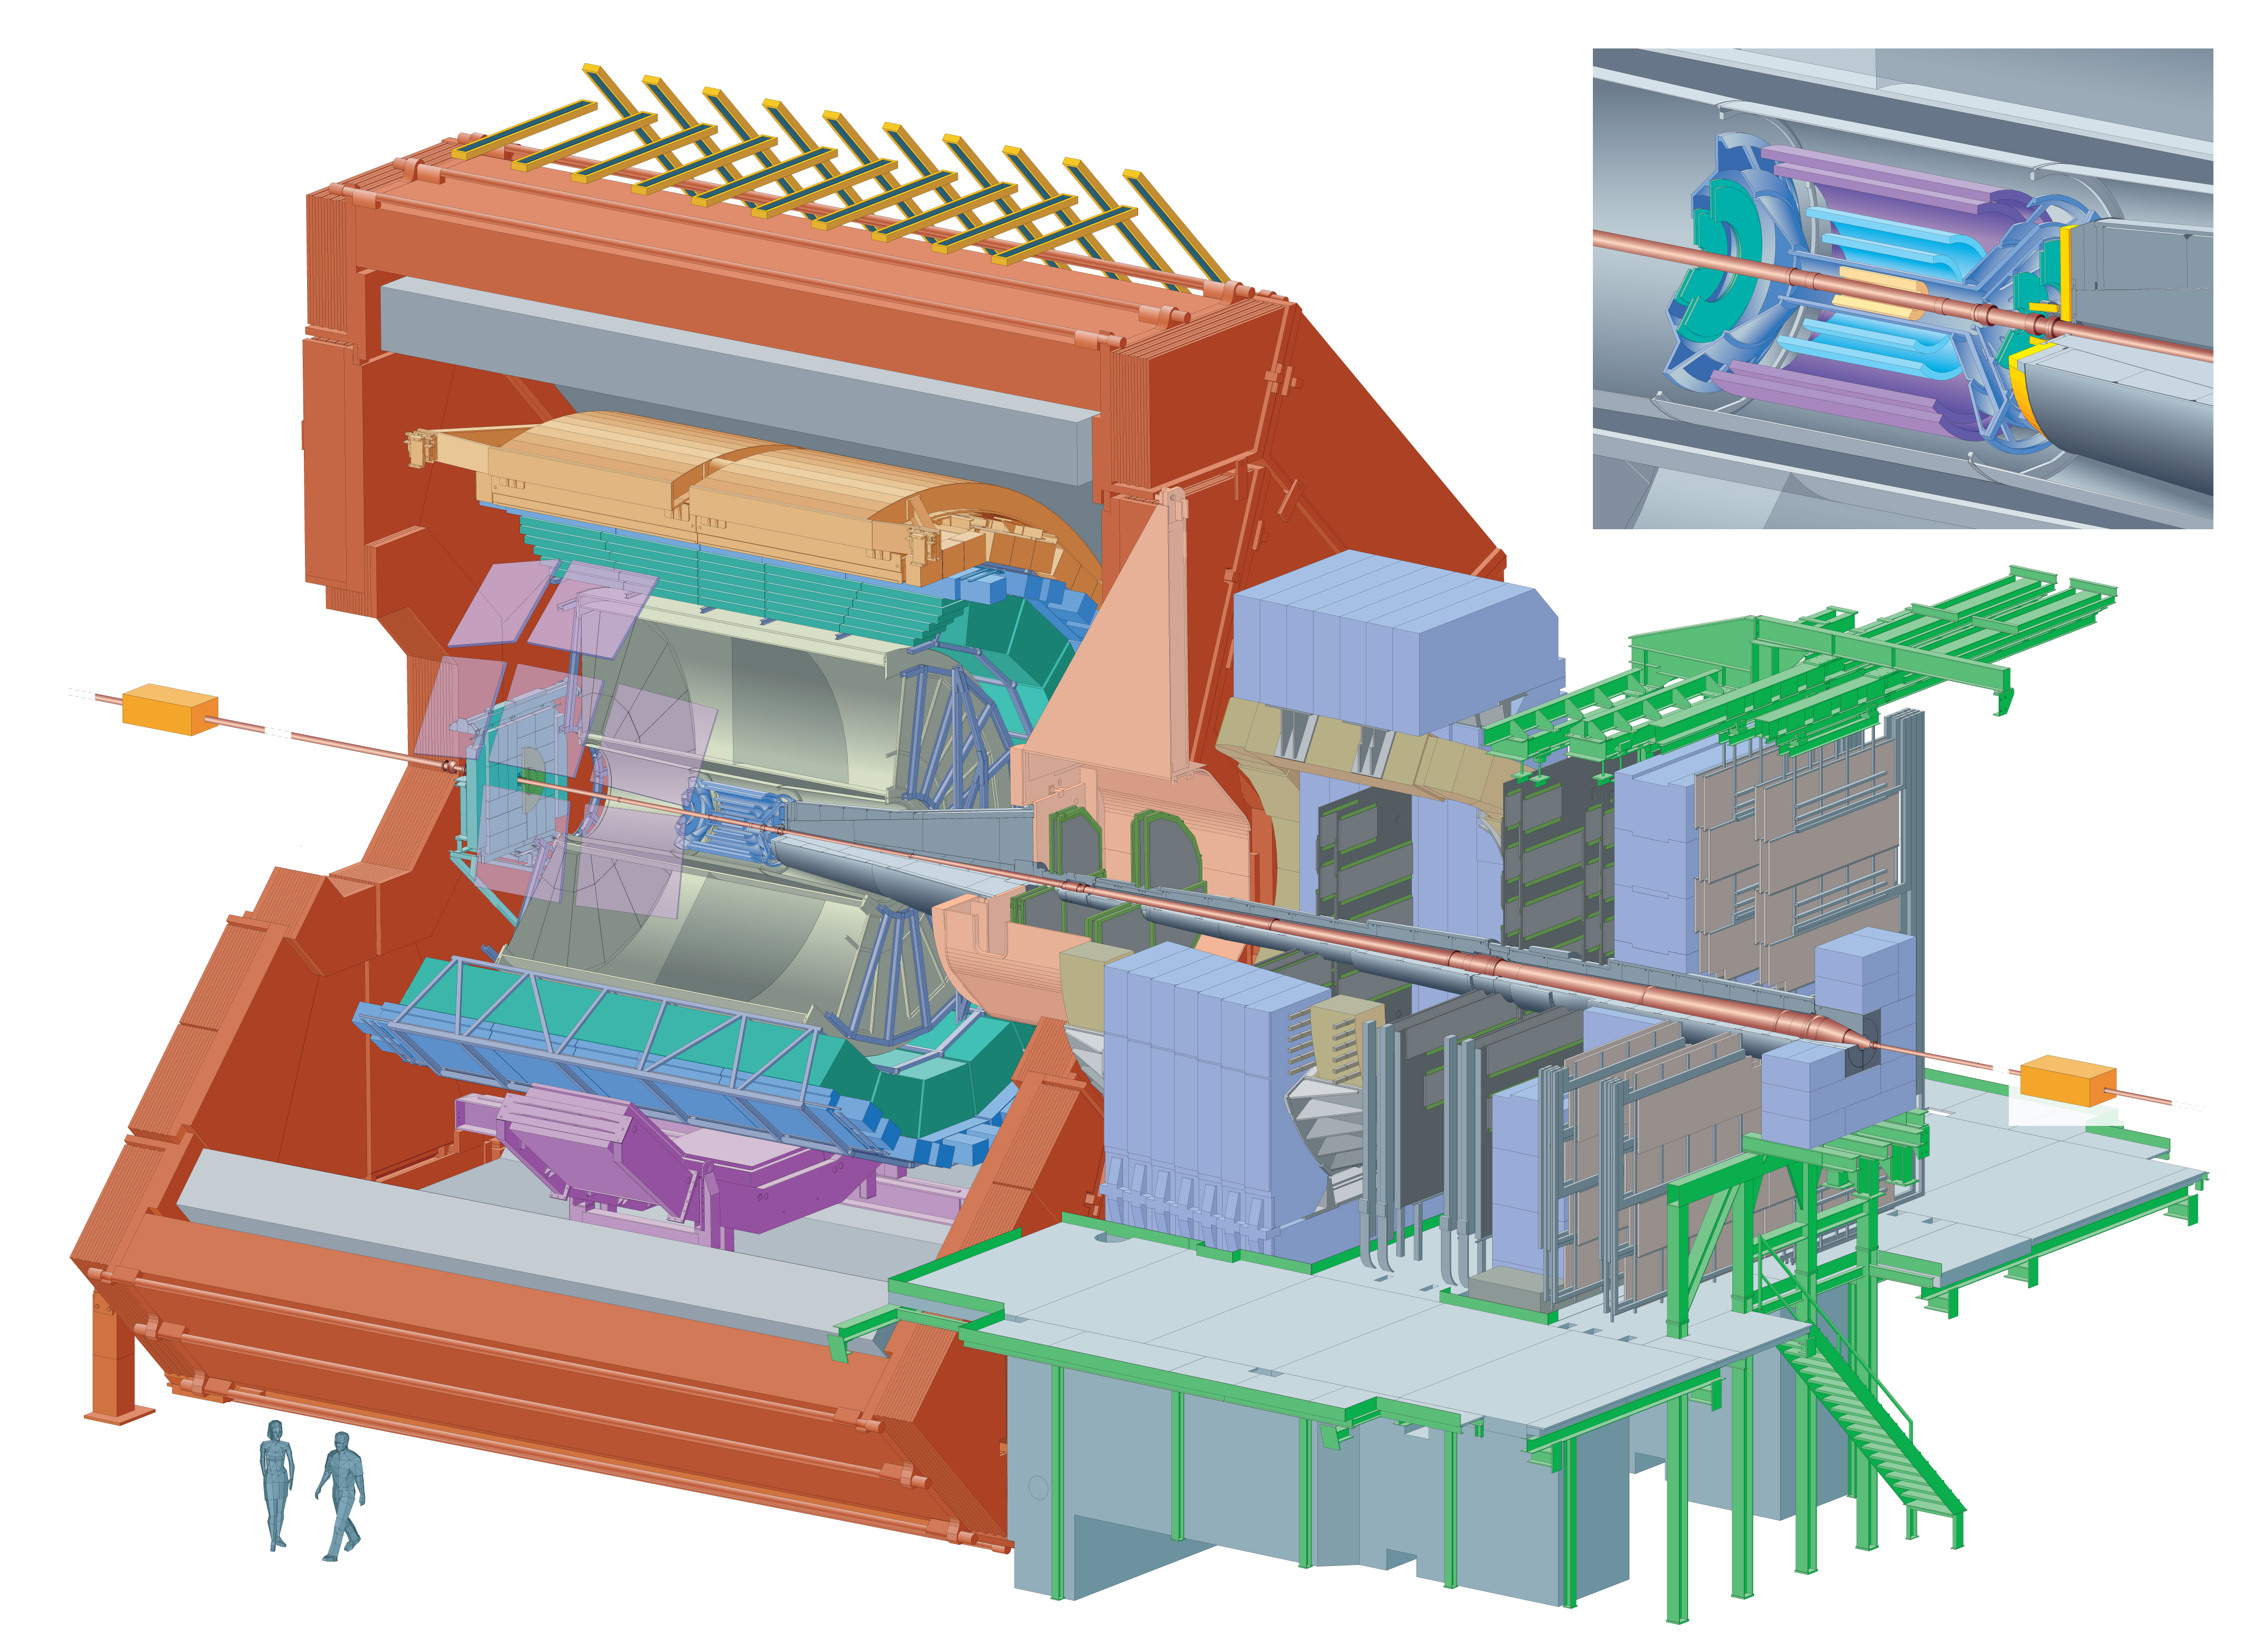
\includegraphics[width=.7\paperwidth]{img/ALICE_Schematics}
\end{frame}

\subsection{D-meson jet tagging}
\begin{frame}{D-meson jet tagging}
\begin{itemize}
\item \Dzero\ meson
\begin{itemize}
\item Mass (PDG): 
\item Lifetime: 
\item Decay: \Dzero$\rightarrow\mathrm{K}^+\pi^-$
\end{itemize}
\item \Dzero\-meson candidates are identified through PID and topological cuts
\item For each D0 candidate we run the jet finding algorithm together with all other reconstructed tracks
\item Combinatorial background coming from random $\mathrm{K}\pi$ pairs needs to be subtracted on a ensemble basis through an invariant mass analysis
\end{itemize}
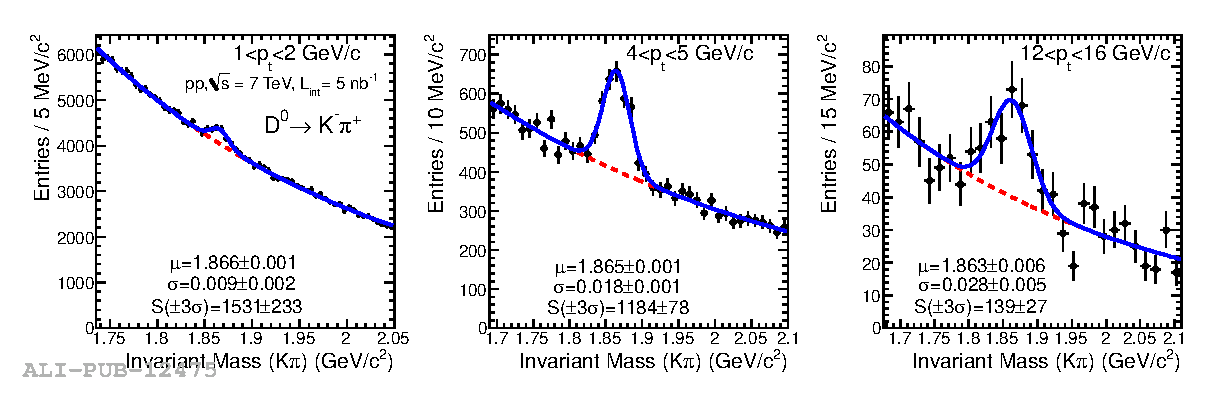
\includegraphics[width=.3\paperwidth]{img/ALICE_D0InvMass}
\end{frame}

\section{Detector Perfomance}

\subsection{D-tagged jet reconstruction efficiency}
\begin{frame}{D-tagged jet reconstruction efficiency}
PYTHIA6 Perugia-2011\\
GEANT3: detailed description of ALICE
\newline
\newline
Steep dependence on the \pt\ of the D meson used to tag jets
\newline
\newline
$\rightarrow$~Due to topological cuts on the secondary vertex, which are tighter at low \ptd\
\newline
\newline
No significant dependence on the \ptchjet: simplifies corrections and reduces systematic uncertainties 
due to the assumptions on fragmentation and interplay with the detector effects
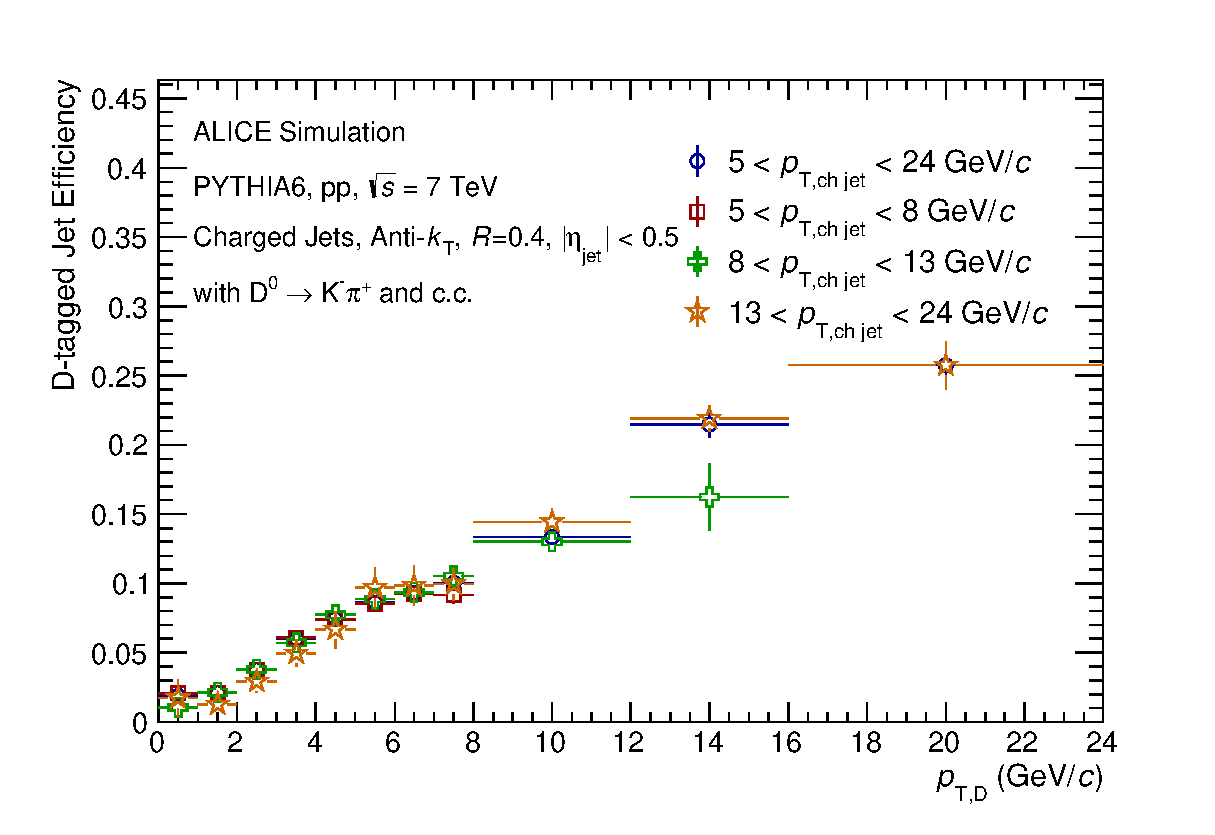
\includegraphics[width=.3\paperwidth]{img/HQ16_Simulation_EfficiencyVsDPt}
\end{frame}

\subsection{JES shift and \pt\ resolution}
\begin{frame}{JES shift and \pt\ resolution}
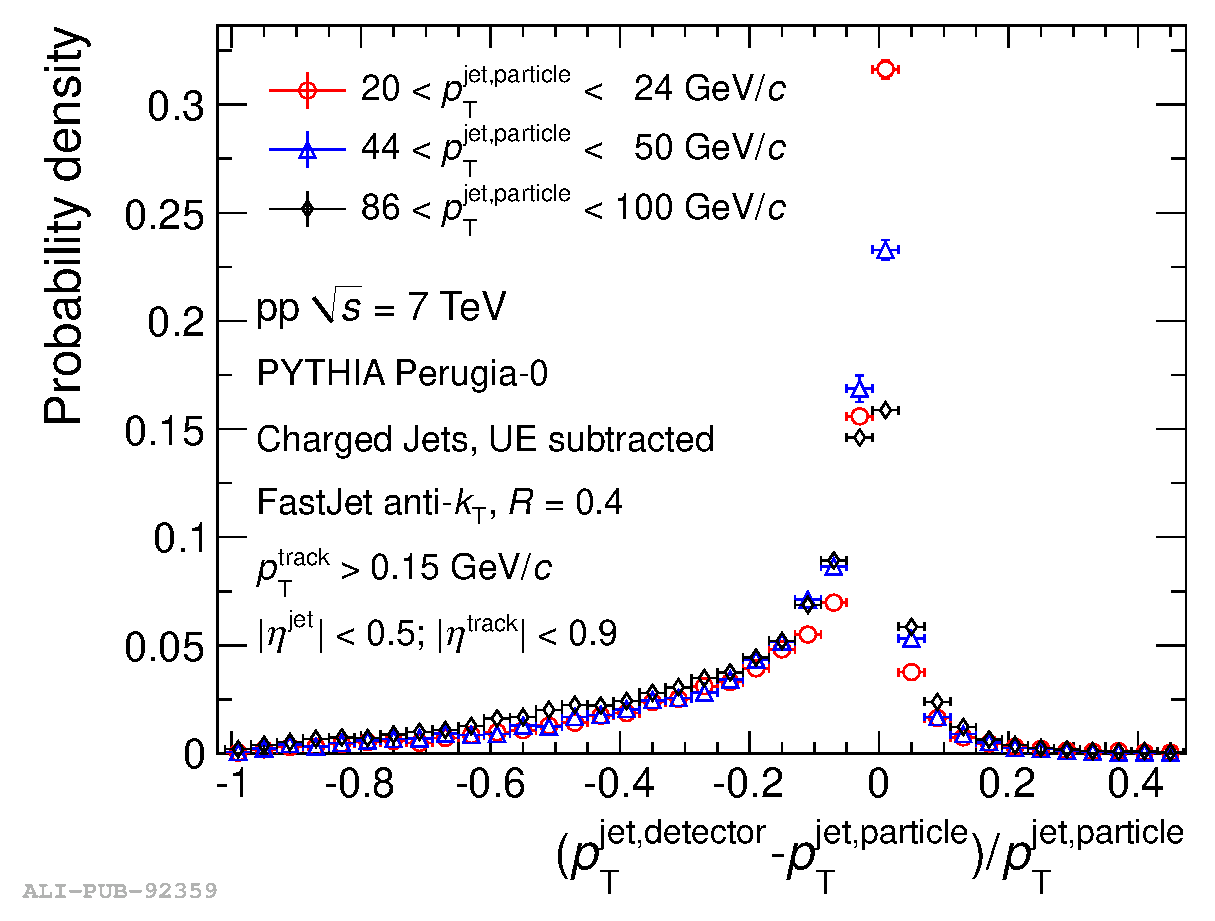
\includegraphics[width=.3\paperwidth]{img/ALICE_JetRes}\quad
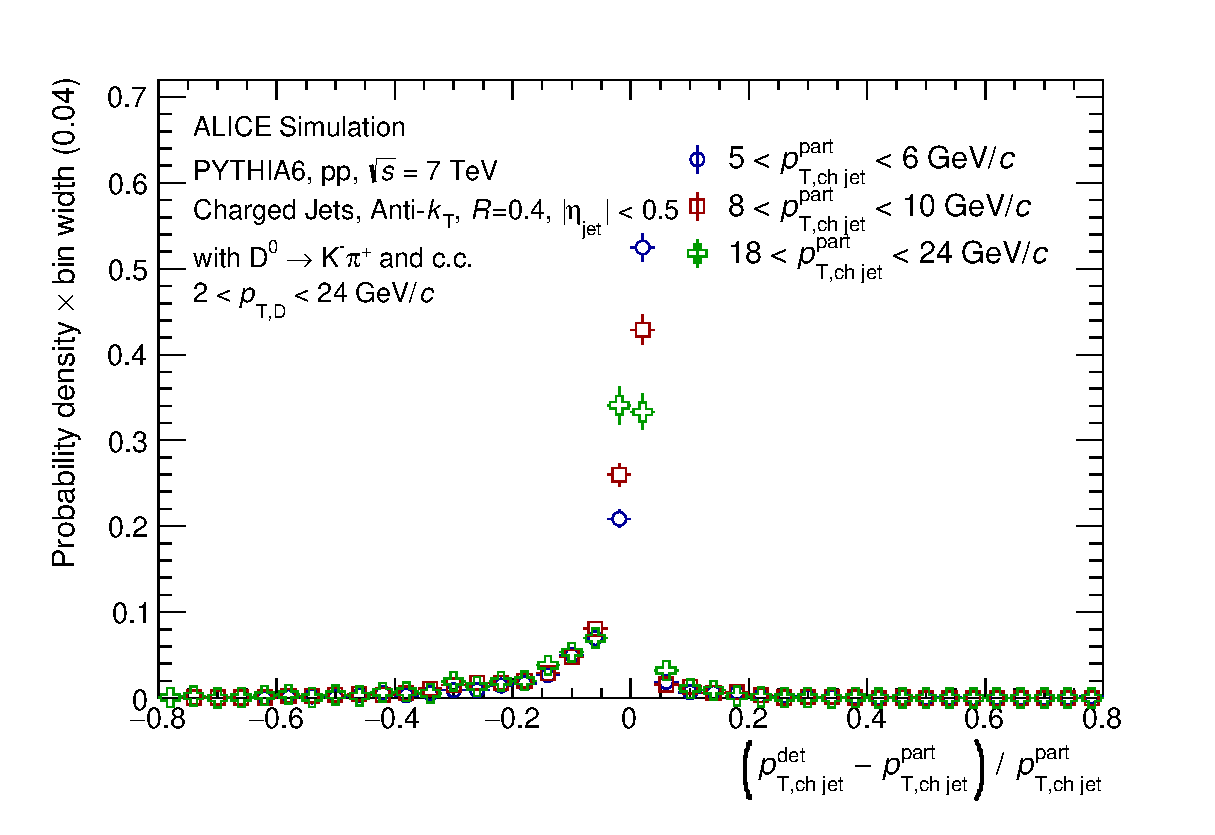
\includegraphics[width=.3\paperwidth]{img/HQ16_Simulation_DetectorResponse}\\
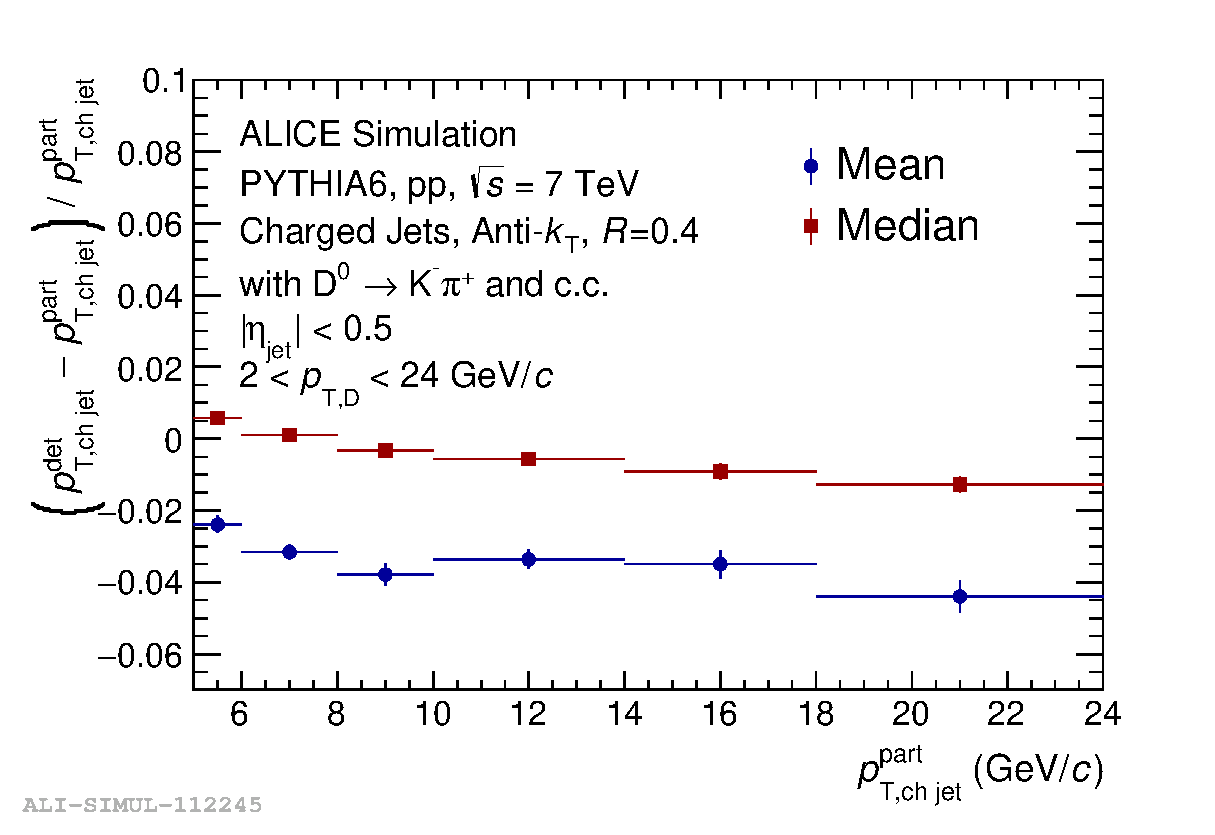
\includegraphics[width=.3\paperwidth]{img/HQ16_Simulation_EnergyScaleShift}\quad
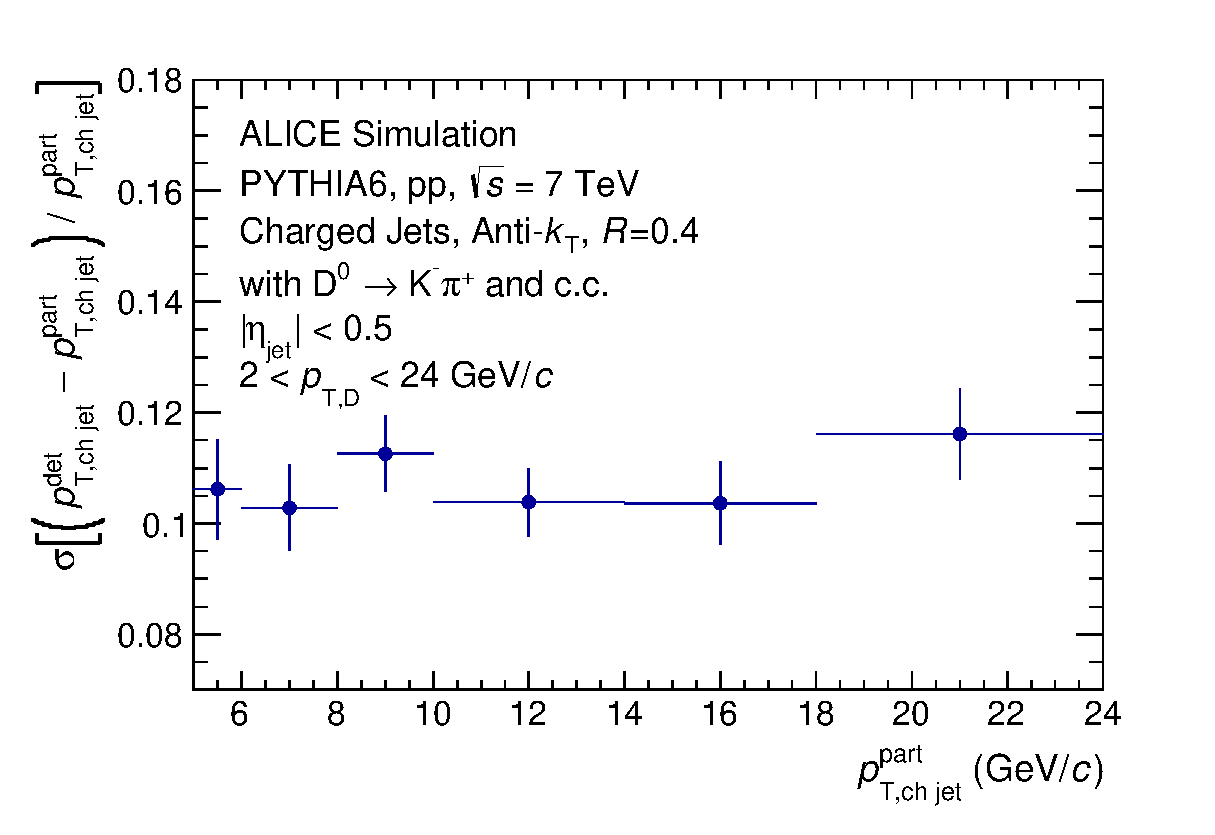
\includegraphics[width=.3\paperwidth]{img/HQ16_Simulation_Resolution}
\newline
Comparable JES shift: $\mu\approx -3\%$
\newline
Slightly better resolution: $\sigma(\mathrm{D-tagged})\approx11\%$, $\sigma(\mathrm{inclusive})\approx17\%$
\end{frame}

\section{Signal Extraction}

\subsection{D-tagged jet signal extraction}
\begin{frame}{D-tagged jet signal extraction}
\begin{itemize}
\item Method 1: invariant mass fit
\begin{itemize}
\item Bin D-tagged jet candidates in \ptchjet
\item Fit invariant mass distributions with a Gaussian (signal) + exponential (background)
\item Extract signal from fit parameters
\end{itemize}
The correction for the D-tagged jet reconstruction efficiency must be applied 
as a weight when filling the invariant mass plots
\pause
\item Method 2: Side-Bands (S-B) / Like-Sign (L-S)
\begin{itemize}
\item Bin D-tagged jet candidates in \ptd
\item Build $N(\ptchjet, \ptd)$ distributions
\item In the peak area for Opposite-Sign (OS) pairs: $|M_{\rm K\pi} - M_{\rm fit}| <2\sigma$\\ $N_{\rm sig+bkg} (\ptchjet, \ptd)$
\item In the SB: $8\sigma <|M_{\rm K\pi} - M_{\rm fit}| < 4\sigma$\\ $N_{\rm bkg, SB} (\ptchjet, \ptd)$
\item In the peak area for LS \\ $N_{\rm bkg, LS} (\ptchjet, \ptd)$
\end{itemize}
\end{itemize}
Efficiency correction before integrating in \ptd: $N_{\rm signal} (\ptchjet)=\sum_{\ptd} \epsilon(\ptd) \times [N_{\rm sig+bkg}(\ptchjet, \ptd) - N_{\rm bkg}(\ptchjet, \ptd)]$
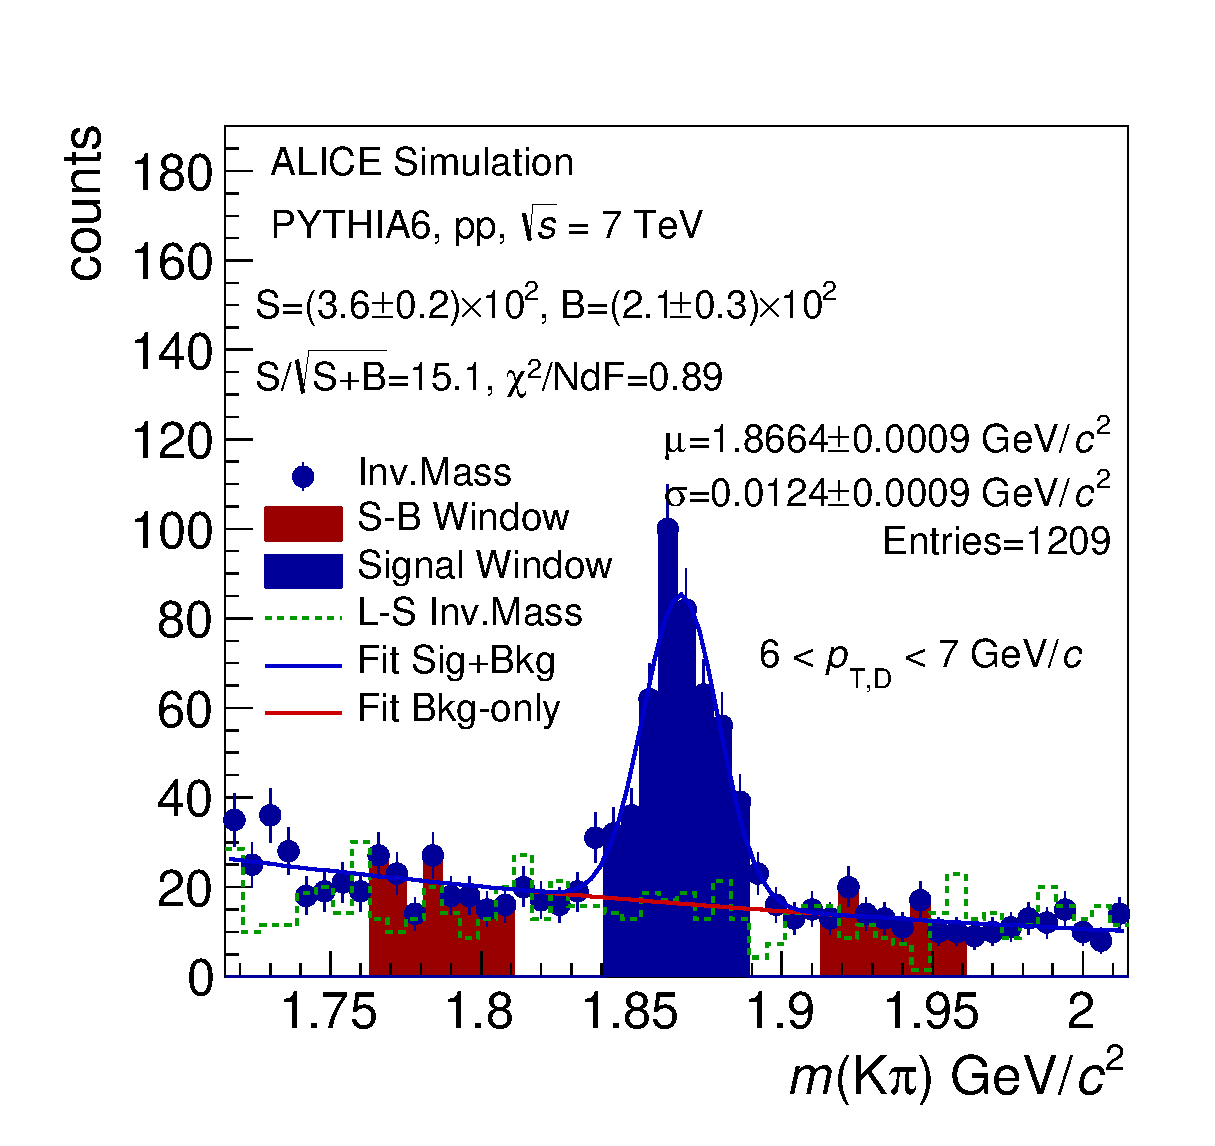
\includegraphics[width=.3\paperwidth]{img/HQ16_Simulation_InvMassSB}
\end{frame}

\subsection{Method comparison}
\begin{frame}{Method comparison}
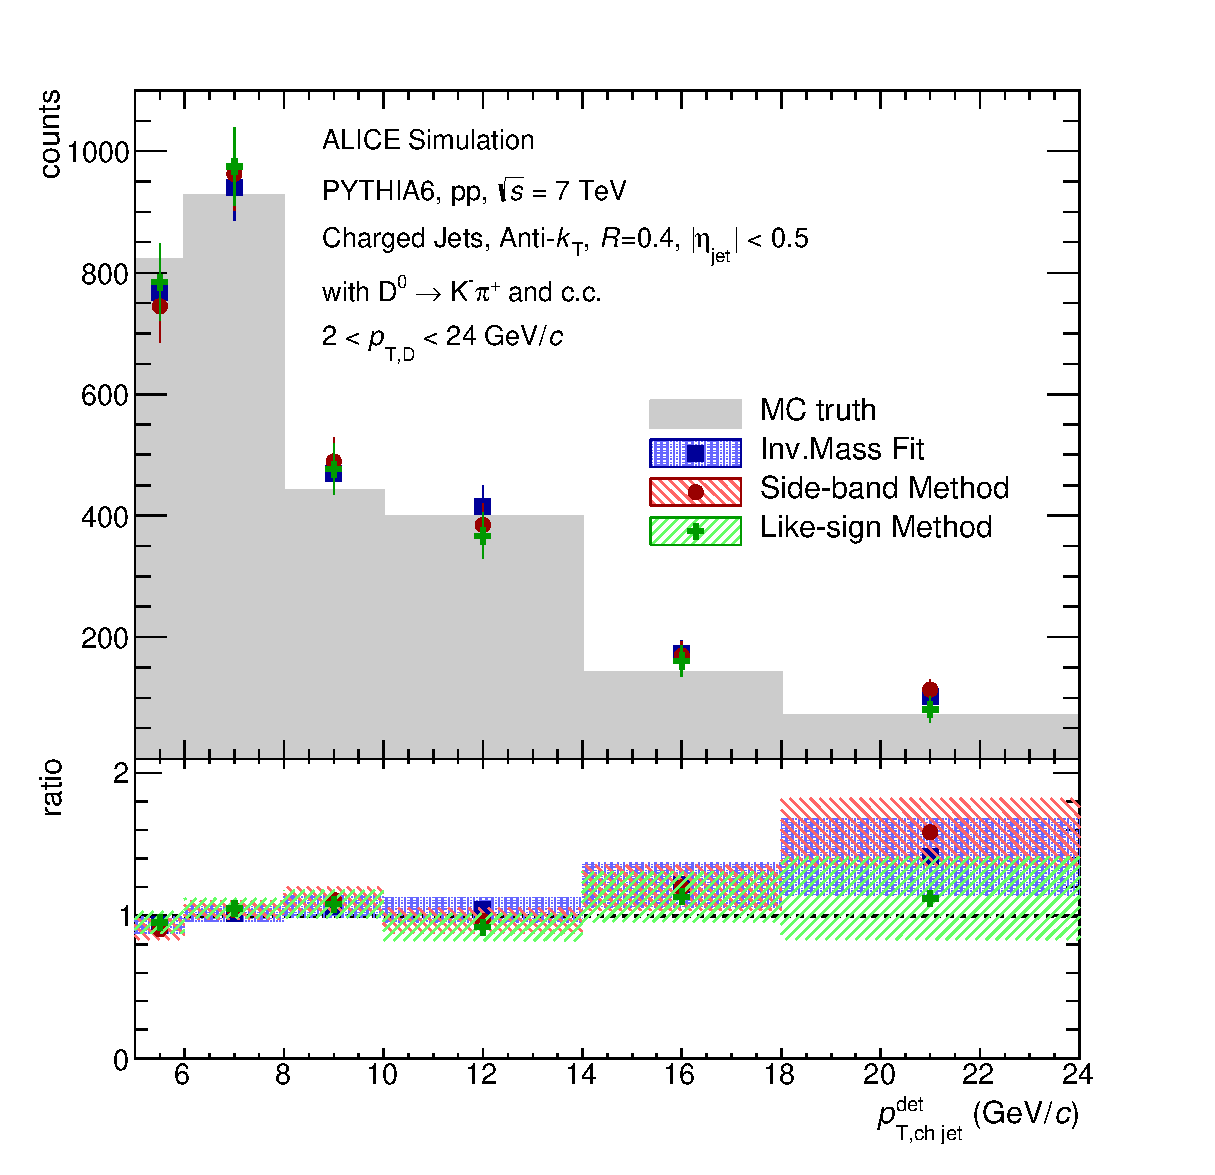
\includegraphics[width=.6\paperwidth]{img/HQ16_Simulation_MethodComparison}
D-tagged jet signal yields extracted using the invariant mass fit, Side-Band and Like-Sign methods are compared with the MC truth
\newline
All methods agree well with the MC truth within their statistical uncertainty
\end{frame}

\subsection{Statistical precision}
\begin{frame}{Statistical precision}
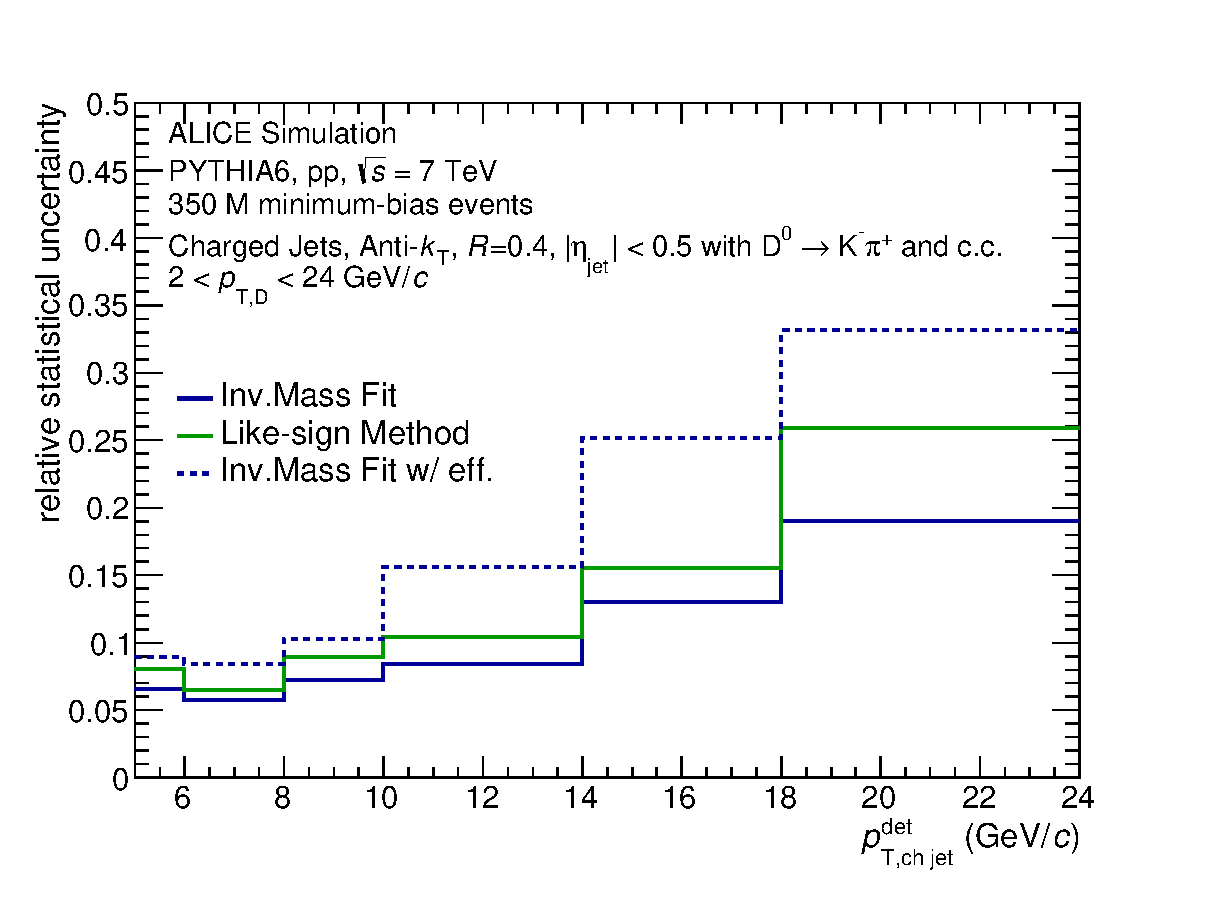
\includegraphics[width=.5\paperwidth]{img/HQ16_Simulation_UncertaintyComparison}
\end{frame}

\section*{Summary}

\subsection*{Conclusions}
\begin{frame}{Conclusions}
\begin{itemize}
\item The measurement of the charm cross-section and of the fragmentation function is of interest for different interconnected fields: 
pQCD, high temperature QCD, high-energy astrophysics
\item 3 different techniques have been developed to extract the D-tagged jet yield:
\begin{itemize}
\item Invariant mass fit in bins of pT,jet
\item Bin counting in the peak area w/ Like-Sign background
\item Bin counting in the peak area w/ Side-Band background
\end{itemize}
\item Proved to be feasible and successfully tested using a detailed simulation of pp collisions and of the ALICE detector performance
\item The pros and cons of each technique is being assessed
\item Now looking forward to finalize the analysis on real data!
\end{itemize}
\end{frame}

\subsection*{Stay Tuned: Work In Progress!}
\begin{frame}{Stay Tuned: Work In Progress!}
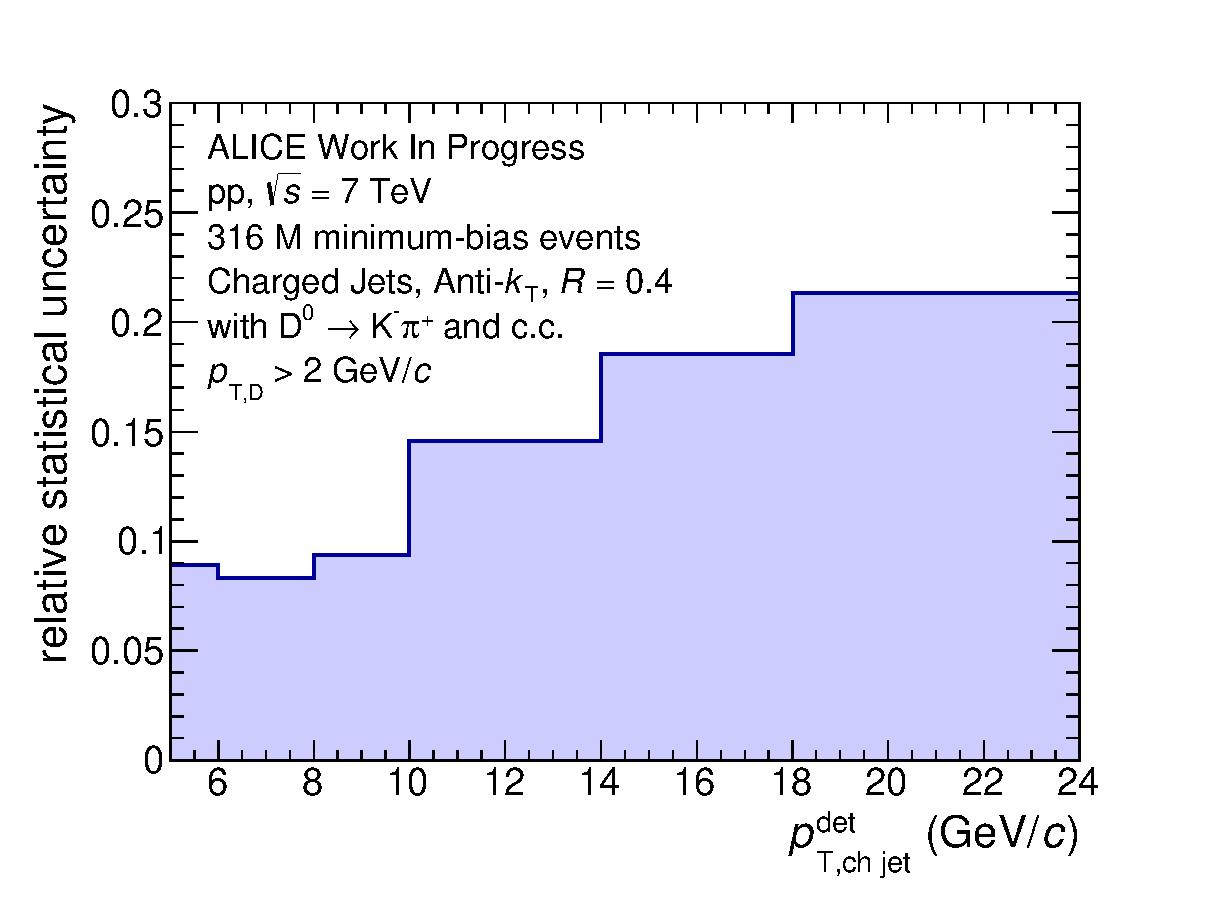
\includegraphics[width=.5\paperwidth]{img/HQ16_WorkInProgress_StatisticalUncertainty}
\begin{itemize}
\item The analysis is being performed using data collected by ALICE with pp collisions at 7 TeV
\item A preliminary look at the available statistics in 2010 data has given promising expectation
\item Look out for new results being made public soon!
\end{itemize}
\end{frame}

% All of the following is optional and typically not needed. 
%\appendix
%\section<presentation>*{\appendixname}
%\subsection<presentation>*{Backup}

%\begin{frame}
 % \frametitle<presentation>{Backup 1}    
%\end{frame}

\end{document}
